\section{Multicore Systeme}

\subsection{Geschwindigkeit auf Prozessor steigern}

\subsubsection{Clockfrequenz erhöhen}

\begin{outline}
    \1 PCB-Design wird sehr anspruchsvoll (Leistungslängen, Reflexionen, etc.)
    \1 Elektrinsche Verlustleistung steigt \textbf{linear} mit Clockfrequenz: $P = f_{\rm cl} \cdot C_L \cdot V_{\rm DD}^2$
    \1 Lichtgeschwindigkeit ist Grenze (Licht legt in $1 \, \nano \second$ $30 \, \centi \meter$ zurück)
\end{outline}

\vspace{0.1cm}

\textrightarrow\ Erhöhung der Clockfrequenz hat eigentlich nur Nachteile

\columnbreak


\subsubsection{Instruction-level parallelism (ILP)}

\begin{outline}
    \1 Parallelismus wird auf \textbf{Instruktionslevel} angestrebt
        \2 Pipelines
        \2 Verschachteln der Instruktionen, um Pipeline möglichst optimal auszulasten
        \2 Vermeiden von Pipline flush durch Vorhersage der Verzweigung (branch prediction)
    \1[-] Branch prediction kann sehr aufwendig werden
    \1[-] Compiler werden komplex
\end{outline}


\subsubsection{Thread-level parallelism (TLP)}

\begin{outline}
    \1 Parallelisierte Einheit ist in der Grössenordnung einer Funktion
        \2 Umfangreichere Stufe der Parallelisierung
    \1 Zugriffe auf gemeinsame Ressourcen (z.B. shared memory) müssen geregelt sein
    \1 Design Issues
        \2 Jeder Thread erzeugt Overhead (Stack, context switch bei single-core Prozessor)
        \2 Nicht beliebig viele Threads möglich
        \2 Bei zu vielen Threads (wenn zusammengehöriges auseinandergenommen wird), werden
            gewisse Daten unnötigerweise shared
\end{outline}


\para{Umsetzung von TLP auf Uniprozessor (single-core)}

\begin{outline}
    \1 Threads werden time-sliced
    \1 Pseudo-TLP
    \1 Context switch notwendig (Umschalten von einem zum anderen Thread)
    \1 \textbf{Ergibt keinen Geschwindigkeitsgewinn}
\end{outline}


\para{Umsetzung von TLP auf Multiprozessor}

\begin{outline}
    \1 Mehrere parallele Prozesse können je einen Thread bearbeiten
    \1 Echter-TLP
    \1 Clockfrequenz kann tiefer gehalten werden
    \1 Einfache Hardware wird multipliziert
    \1 Datenaustausch zwischen Prozessen muss geregelt werden, z.B. mit Message Passing / Shared Memory
\end{outline}


\subsection{Speicherorganisation auf Multicore Prozessor}

\begin{minipage}[t]{0.45\columnwidth}
    \raggedright
    \para{Shared Memory}

    \begin{outline}
        \1 Alle Prozessoren nutzen einen gemeinsamen Speicher
            \2 Kann zum Falschenhals werden
    \end{outline}
\end{minipage}
\hfill
\begin{minipage}[t]{0.53\columnwidth}
    \raggedright
    \para{Distributed Memory}

    \begin{outline}
        \1 Jeder Prozessor hat eigenen lokalen Speicher
            \2 Braucht Mechanismus für Datenaustausch, z.B. Message Parsing
    \end{outline}
\end{minipage}


\subsubsection{Multicore Prozessor}

\begin{outline}
    \1 Spezieller Multiprozessor \textrightarrow\ alle Cores (Prozessoren) auf demselben Chip
    \1 MIMD (Multiple Instructions Multiple Data)
    \1 Komplexe Speicherorganisation
        \2 Caches, per core local memory, Shared Memory
    \1 Homogene vs. heterogene Multicore Prozessoren
\end{outline}


\subsubsection{Embedded Computing vs. PC/Enterprise Computing}


\para{PC / Enterprise Computing}

\begin{outline}
    \1 Meist \textbf{homogene} Multicores
        \2 Gesamtaufgabe aufteilen für optimale Ausühtungszeit \textrightarrow\ Amdahl's Law
    \1 Parallelisierung möglichst automatisiert (z.B. durch Compiler)
\end{outline}

\para{Embedded Computing}

\begin{outline}
    \1 Oft \textbf{heterogene} Multicores
        \2 ARM Core für administrative Aufgaben
        \2 ein bis mehrere DSPs für effiziente mathematische Berechnungen
        \2 Aufteilung ergibt sich von selbst
\end{outline}


\subsection{Amdahl's Law}

Amdahl's Law beschreibt den theoretisch mögichen Speedup $S$ eines parallellen Tasks, wenn dieser
auf mehrere Cores (Prozessoren) aufgeteilt wird. \\
\textbf{Hinweis:} Typischerweise bleibt ein Teil des Tasks sequenzell. Dieser kann nicht aufgeteilt werden
und \textbf{limitiert} somit den möglichen Speedup.

\vspace{0.1cm}

% \begin{minipage}[t]{0.48\columnwidth}
%     $$ S(n) = \frac{1}{1 - p + \frac{p}{n}} $$
%     $$ S \leq \frac{1}{1-p} $$
        
%     \begin{tabular}{ll}
%         $S$     & Speedup (Faktor, z.B. 4.0)            \\
%         $p$     & Parallel Portion (z.B. 0.5 = 60 \%)   \\
%         $n$     & Anzahl Cores                  
%     \end{tabular}
% \end{minipage}
% \hfill
% \begin{minipage}[t]{0.48\columnwidth}
%     $$ S(n) = \frac{T}{t_s + \frac{t_p}{n}} $$
%     $$ S \leq \frac{T}{T - t_p} = \frac{T}{t_s} $$

%     \begin{tabular}{ll }
%         $T$     & Totale Ausführungszeit        \\
%         $t_p$   & Parallele Ausführungszeit     \\
%         $t_s$   & Serielle Ausführungszeit  
%     \end{tabular}
% \end{minipage}

\begin{minipage}[c]{0.25\columnwidth}
    $$ S(n) = \frac{1}{1 - p + \frac{p}{n}} $$
    $$ S \leq \frac{1}{1-p} $$
\end{minipage}
\hfill
\begin{minipage}[c]{0.25\columnwidth}
    $$ S(n) = \frac{T}{t_s + \frac{t_p}{n}} $$
    $$ S \leq \frac{T}{T - t_p} = \frac{T}{t_s} $$
\end{minipage}
\hfill
\begin{minipage}[c]{0.48\columnwidth}
    \begin{tabular}{ll}
        $S$     & Speedup (Faktor, z.B. 4.0)            \\
        $p$     & Parallel Portion (z.B. 0.6 = 60 \%)   \\
        $n$     & Anzahl Cores                          \\
        $T$     & Totale Ausführungszeit                \\
        $t_p$   & Parallele Ausführungszeit             \\
        $t_s$   & Serielle Ausführungszeit  
    \end{tabular}
\end{minipage}


\subsection{Memory Hierarchy}

\begin{center}
    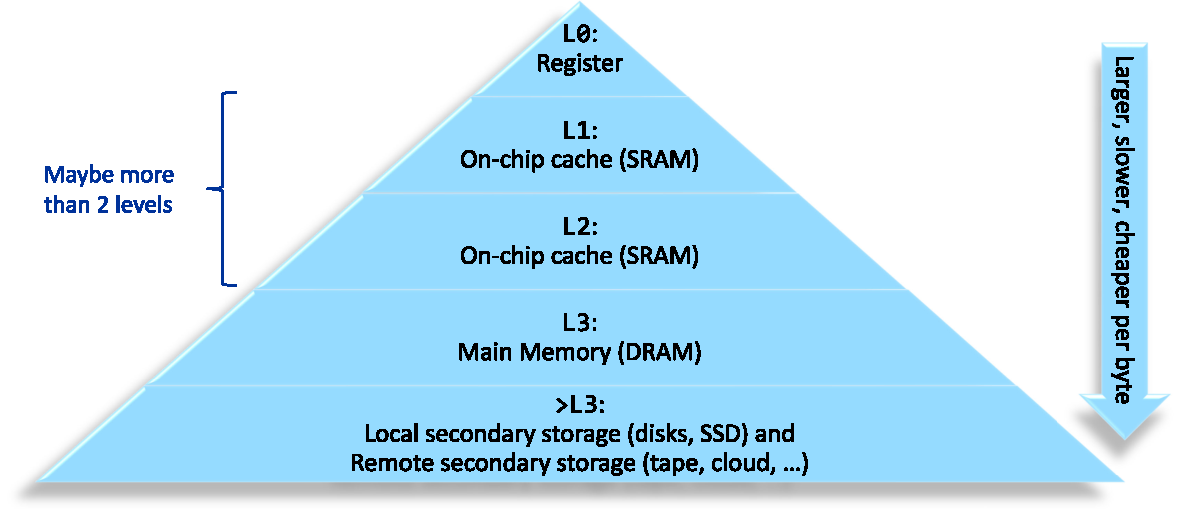
\includegraphics[width=0.88\columnwidth]{images/multiprocessor_memory.pdf}
\end{center}


\subsection{Cache-Speicher}

\begin{outline}
    \1 Für Prozessor versteckte, schnelle Speicher \textrightarrow\ liegen zw. Prozessor und Hauptspeicher
    \1 \textbf{Führen Kopie von häufig benötigten Hauptspeicherdaten}
        \2 Nutzen zeitliche und örtliche Lokalität von Programmen aus
    \1 \textbf{Cache Hit:} Vom Prozessor benötigte Hauptspeicherdaten sind im Cache
        \2 Schnellerer Zugriff möglich
    \1 \textbf{Cache Miss:} Daten müssen aus Hauptspeicher geholt werden
 \end{outline}

 $$ \boxed{ \text{Mittlere Zuegriffszeit} = (\text{Hit Time}) \cdot (\text{Hit Rate}) + (\text{Miss Penalty}) \cdot (\text{Miss Rate}) } $$


 \begin{tabular}{l c l}
    (Hit Time)      & $=$   & (Zeit zur Bestimmung von Hit oder Miss) $+$   \\
                    &       & (Speicherzugriffszeit auf Cache)              \\
    (Miss Penalty)  & $=$   & (Zeit zur Bestimmung von Hit oder Miss) $+$   \\
                    &       & (Zeit zum Ansprechen der nächsten Ebene) $+$  \\
                    &       & (Zeit zum Übertragen von der nächsten Ebene)
 \end{tabular}      


\subsubsection{Zeitliche / örtliche Lokalität}

\para{Zeitliche Lokalität (Temporal locality)}

\begin{outline}
    \1 Soeben verwendete Daten / Instruktionen werden mit hoher \myul{Wahrscheinlichkeit} bald wieder verwendet
        \2 \textbf{Caches nutzen zeitliche Lokalität aus}
\end{outline}


\para{Örtliche Lokalität (Spatial locality)}

\begin{outline}
    \1 Bei soeben verwendete Daten / Instruktionen werden mit hoher \myul{Wahrscheinlichkeit} auch benachbarte Daten / Instruktionen verwendet
        \2 Caches: Wenn auf eine bestimmte Adresse das erste Mal zugegriffen wird, werden nicht nur die Daten von dieser Adresse ins Cache 
            geladen, sondern ein Speicherblock bestimmter Grösse um diese Adresse herum
\end{outline}

\vspace{0.1cm}

\textrightarrow\ Cache ist reine Wahrscheinlichkeit! \textrightarrow\ Hoffen, dass Daten dort sind...


\subsection{Cache Ersetzungsstrategien}

Es gibt mehrere Strategien, um zu ermitteln, welche Daten aus dem Cache entfernt werden sollen, um Platz für neue Daten zu schaffen.
Dabei ist zu beachten, dass bei jeder Eretzung allenfalls Daten in die \textbf{nächste Stufe zurückgeschrieben} werden müssen.
Dies ist immer dann der Fall, wenn das \textbf{Dirty Bit} (Signal, dass Cache-Daten geändert haben) gesetzt ist.

\vspace{0.1cm}

\begin{outline}
    \1 \textbf{LRU (Least Recently Used)} \textrightarrow\ häufige Strategie
        \2 Bei Zugriff muss zusätzlich ein Timestamp gespeichert werden
    \1 \textbf{LFU (Least Frequently Used)}
        \2 Bei Zugriff muss Counter gespeichert werden (wie oft Daten gebraucht wurden)
    \1 \textbf{FIFO (First In First Out)}
        \2 doof, wenn man Daten oft braucht, diese aber schon lange im Cache liegen
    \1 \textbf{Random}
\end{outline}


\subsection{Caches in Echtzeitsystemen}

\begin{outline}
    \1 In (harten) Echtzeitsystemen ist \textbf{Worst Case Execution Time (WCET)} wichtig
        \2 \textbf{WCET mit Cache} immer \textbf{schlechter} als ohne Cache!\\
        \textrightarrow\ wegen Bestimmung ob Hit oder Miss
    \1 Wegen steigender WCET sind Caches in Echtzeitsystemen \textbf{allenfalls ungeeignet}
\end{outline}

\vspace{0.1cm}

\textrightarrow\ WCET tritt so selten ein, dass Caches trotzdem die schnellste Option sein sollten (wegen gesenkter \textbf{mittlerer Zugriffszeit})


\subsection{Cache Coherence}

Bei Multicore-Systemen können \textbf{Kopie derselben Daten in mehreren Cashes} liegen. \\
Cache Coherence beschreibt, wie ein Cache eines Cores \textbf{erfährt}, dass ein anderer Core diese \textbf{Daten geändert} hat. 
Cache Coherence kann mit verschiedenen Protokollen oder auch mit Hardware-Unterstützung umgesetzt werden.


\subsubsection{MESI Cache Coherence Protocol}

Jede 'cache line' hat einen der folgenden Zustände:

\vspace{0.1cm}

\begin{minipage}[t]{0.48\columnwidth}
    \raggedright
    \begin{outline}
        \1 \textbf{Modified (M)}
            \2 Lokale Kopie modifiziert, keine Kopien in anderen Caches
            \2 Memory is 'stale' (dirty)
        \1 \textbf{Exclusive (E)}
            \2 Keine Kopien in anderen Caches
            \2 Memory up to date
    \end{outline}
\end{minipage}
\hfill
\begin{minipage}[t]{0.48\columnwidth}
    \raggedright
    \begin{outline}
        \1 \textbf{Shared (S)}
            \2 Unmodifizierte Kopien in anderen Cashes möglich
            \2 Memory up to date
        \1 \textbf{Invalid (I)}
            \2 Cache line nicht benutzt
    \end{outline}
\end{minipage}


\subsubsection{Cache Coherence mittels HW-Unterstützung}

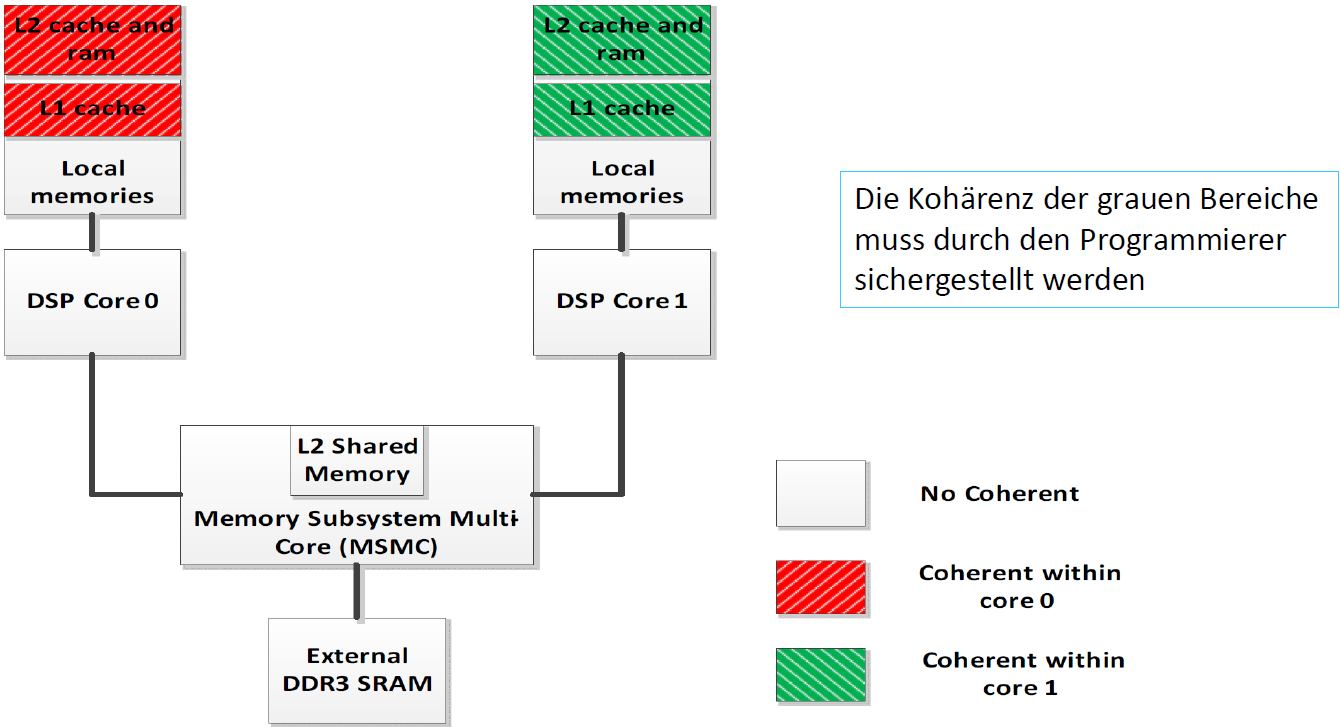
\includegraphics[width=\columnwidth]{images/multicore_cache_coherence_HW.png}


\subsection{Programmierung von Shared Memory in C und C++}

\begin{minipage}[t]{0.56\columnwidth}
    \begin{outline}
        \1 Beide Cores haben \textbf{eigenen} Adressbereich
        \1 \mylstbox[morekeywords={[3], sharedVariable}]{sharedVariable} liegt auf \textbf{fester Adresse in Shared Memory} und wird von
            beiden Cores genutzt
        \1 Zugriff auf \mylstbox[morekeywords={[3], sharedVariable}]{sharedVariable} muss \textbf{synchronisiert} werden
        \1 Zwischen Cores und \mylstbox[morekeywords={[3], sharedVariable}]{sharedVariable} können mehrere Caches liegen
        \1 \textbf{Jeder Core muss} \mylstbox[morekeywords={[3], sharedVariable}]{sharedVariable} \textbf{für sich definieren} \textrightarrow\ \mylstbox{volatile}
    \end{outline}

    \vspace{0.2cm}
    \mylstbox{volatile} hat Einfluss zur Compile-time und 'verbietet' dem Compiler das Anlegen einer Kopie in einem Arbeitsregister
\end{minipage}
\hfill
\begin{minipage}[t]{0.42\columnwidth}
    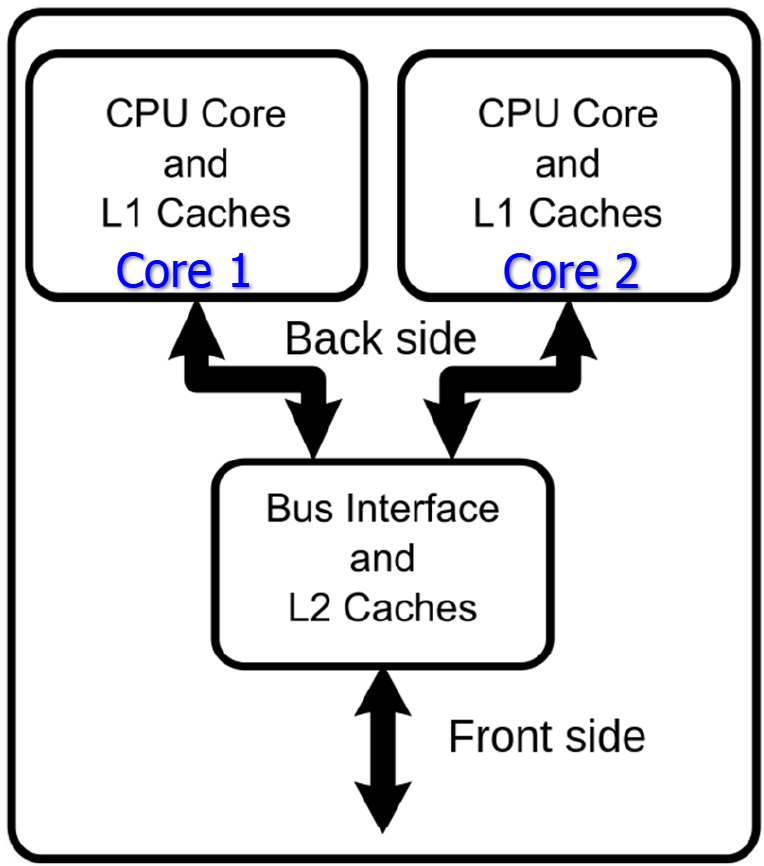
\includegraphics[width=\columnwidth, align=t]{images/multicore_shared_memory.png}
\begin{lstlisting}[belowskip=0mm, morekeywords={[3], sharedVariable}]
    volatile int sharedVariable;
\end{lstlisting}
\end{minipage}


\subsubsection{volatile Variablen}

\begin{outline}
    \1 \textbf{Alle Variablen, die ausserhalb des Programmkontextes des Prozessors/Threads geändert werden können müssen \lstinline|volatile| sein!}
        \2 Variablen, die (speziell bei Embedded Systems) ein Hardwareregister darstellen
        \2 Globale Variablen, auf die in mehreren Threads zugegriffen wird (concurrency)
        \2 Globale Variablen, die in einer ISR geändert werden
        \2 Shared Variablen, die von einem anderen Prozessor/Core geändert werden können
\end{outline}


\subsection{Speicherzugriff zur Laufzeit}

\begin{outline}
    \1 Dank \mylstbox{volatile} besteht generierter Maschinencode aus \textbf{explizitem Speicherzugriff}
        \2 soll so schnell wie möglich sein
        \2 Hoffnung: Daten sind in prozessornahem Cache
    \1 Geschwindigkeitsgewinn erst ab zweitem Zugriff (erst dann sind Daten im Cache) \\
        \textrightarrow\ \textbf{Daten, auf die nur einmal zugegriffen wird, sollen nicht gecached werden!}
    \1 \mylstbox{volatile} löst Cache Coherence Problem nicht
        \2 \textbf{\mylstbox{volatile} ist notwendig, aber nicht hinreichend!}
\end{outline}


\subsection{Datenkonsistenz}

Oft tritt folgendes Szenario ein: 

\vspace{0.1cm}

\begin{itemize}
    \item System empfängt Daten (z.B. ein Bild) und schreibt sie in Buffer
    \item Daten werden gefiltert (z.B. Image Processing) und wieder ausgegeben
\end{itemize}

\vspace{0.1cm}

Es stellt sich die Frage: Wie kann \textbf{verhindert werden}, dass der Filterschritt \textbf{inkonsistente Daten im Buffer} hat, weil der
Empangsteil laufend Daten in den Buffer schreibt?

\vspace{0.2cm}

\begin{minipage}[t]{0.45\columnwidth}
    \para{Schlechte Lösung}

    \begin{itemize}
        \item Buffer wird synchronisiert (z.B. mit Semaphoren)
        \item[-] Overhead, strenge Serialisierung
    \end{itemize}
\end{minipage}
\hfill
\begin{minipage}[t]{0.52\columnwidth}
    \para{Triviale Lösung}

    \begin{itemize}
        \item Empfangsbuffer wird in zweiten Buffer kopiertk sobald Daten fertig empfangen sind
        \item[-] Kopieren ist teuer
    \end{itemize}
\end{minipage}


\para{Vernünftige Lösung für Datenkonsistenz -- Ping Pong Buffer}

\begin{itemize}
    \item Zwei identische Buffer definieren
    \item Ein Core (Master) bestimmt, in welchen Buffer die Daten geschrieben werden
    \item Nach Empfangen der Daten übergibt Master dem Filterschritt einen \textbf{Pointer} auf 'Daten-Buffer'
    \item Master übergibt Sender der Daten \textbf{Pointer auf zweiten Buffer}, damit Daten nun dort geschrieben werden \\
        \textrightarrow\ Ping Pong zwischen den zwei Buffern
\end{itemize}

\vspace{0.1cm}

Noch besser ist es, wenn der Empfang der Daten über DMA (Direct Memory Access) erfolgt. \\
\textrightarrow\ DMA-Einheit braucht nur Ziel-Pointer und Byte Counter

